\setchapterpreamble[u]{\margintoc}
\chapter{Introduction}
\labch{intro}


Current trends in collection of data are increasing, with more and more human activities producing machine-readable information, such as product reviews \sidecite[1.8cm]{fang2015sentiment}, posts on social media \sidecite[2.7cm]{balaji2021machine}, medical images \sidecite[3.45cm]{willemink2020preparing}, industrial machinery sensor data \sidecite[4.72cm]{gao2015survey}, and more. Automatic processing of data makes it easier to obtain  results fast and saves hours of human labor which can be freed for other purposes or dedicated to tasks which cannot be automated. The speed provided by current computation resources also opens new possibilities for leveraging the available data, achieving extraction and manipulation of information at levels infeasible by human hand.

The study of problems, tools and solutions related to data integration, processing and analysis has been recently known as data science \sidecite[1.5cm]{dhar2013data}, a field which overlaps branches of mathematics, statistics and computer science, among other disciplines. Current data science applications are present everywhere, from the most industrial settings to direct final user access, and range from machinery fault detection \sidecite{carvalho2019systematic}, to medical diagnosis assistance \sidecite{erickson2017machine}, customer loyalty in retail \sidecite{ma2020machine} and photograph enhancing \sidecite{wang2020deep}.

The general objective in a data science problem is to model a real world scenario based on the collected data and use the resulting model to provide some information to the end user, for example, a category or label, a ranking, an association or a transformed version of the original data. This is a process that encompasses all steps from data acquisition, to its preparation, processing and analysis. In this context, a wide variety of computer algorithms are used to manipulate and process data. The study and development of these techniques that allow machines to distill knowledge from data are known as \textit{machine learning}.

\section{Problem setting}

There are several stages that compose the process of solving a data science problem, represented visually in Figure~\ref{fig:kdd}. A great part of the time spent, usually the longest, consists in preparing and preprocessing the available data in order for the posterior learning techniques to extract the maximum possible amount of information and ensure the new knowledge is valid \sidecite{domingos2012few}. There exist several traits of the data that can be manipulated to facilitate the work of learning algorithms: missing values, noisy instances, class imbalance, among others \sidecite{garcia2015data}.

\begin{figure}
    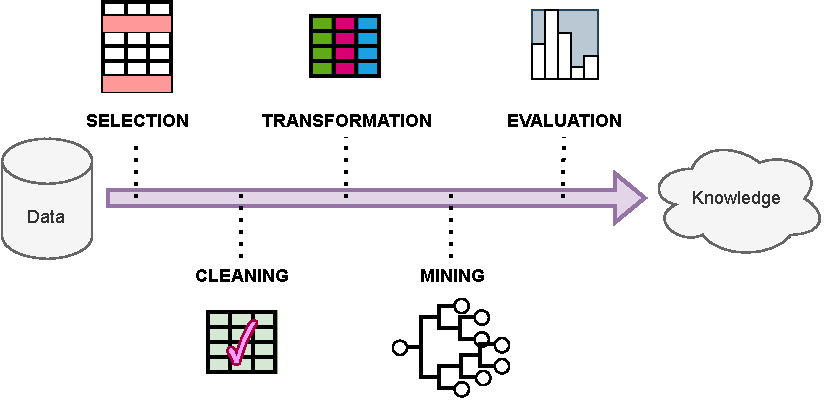
\includegraphics[width=\linewidth]{images/kddprocess.pdf}
    \caption{\label{fig:kdd}Process of knowledge discovery in databases (KDD)}
\end{figure}

The set of features, that is, the specific representation of each instance in a dataset, is one aspect which machine learning models can be specially sensitive to.

Features that may characterize an event or object adequately for humans may not be ideal for machines to process. For example, a string of text may have meaning for a reader but for the machine it is just a sequence of characters whose semantics are not easily processed in that format. Similarly, an image can be expressed as a series of color values which, if shown on a screen, will display something intelligible for a person's eye, but those values do not hold direct relation to what is contained in the image itself.

\begin{marginfigure}
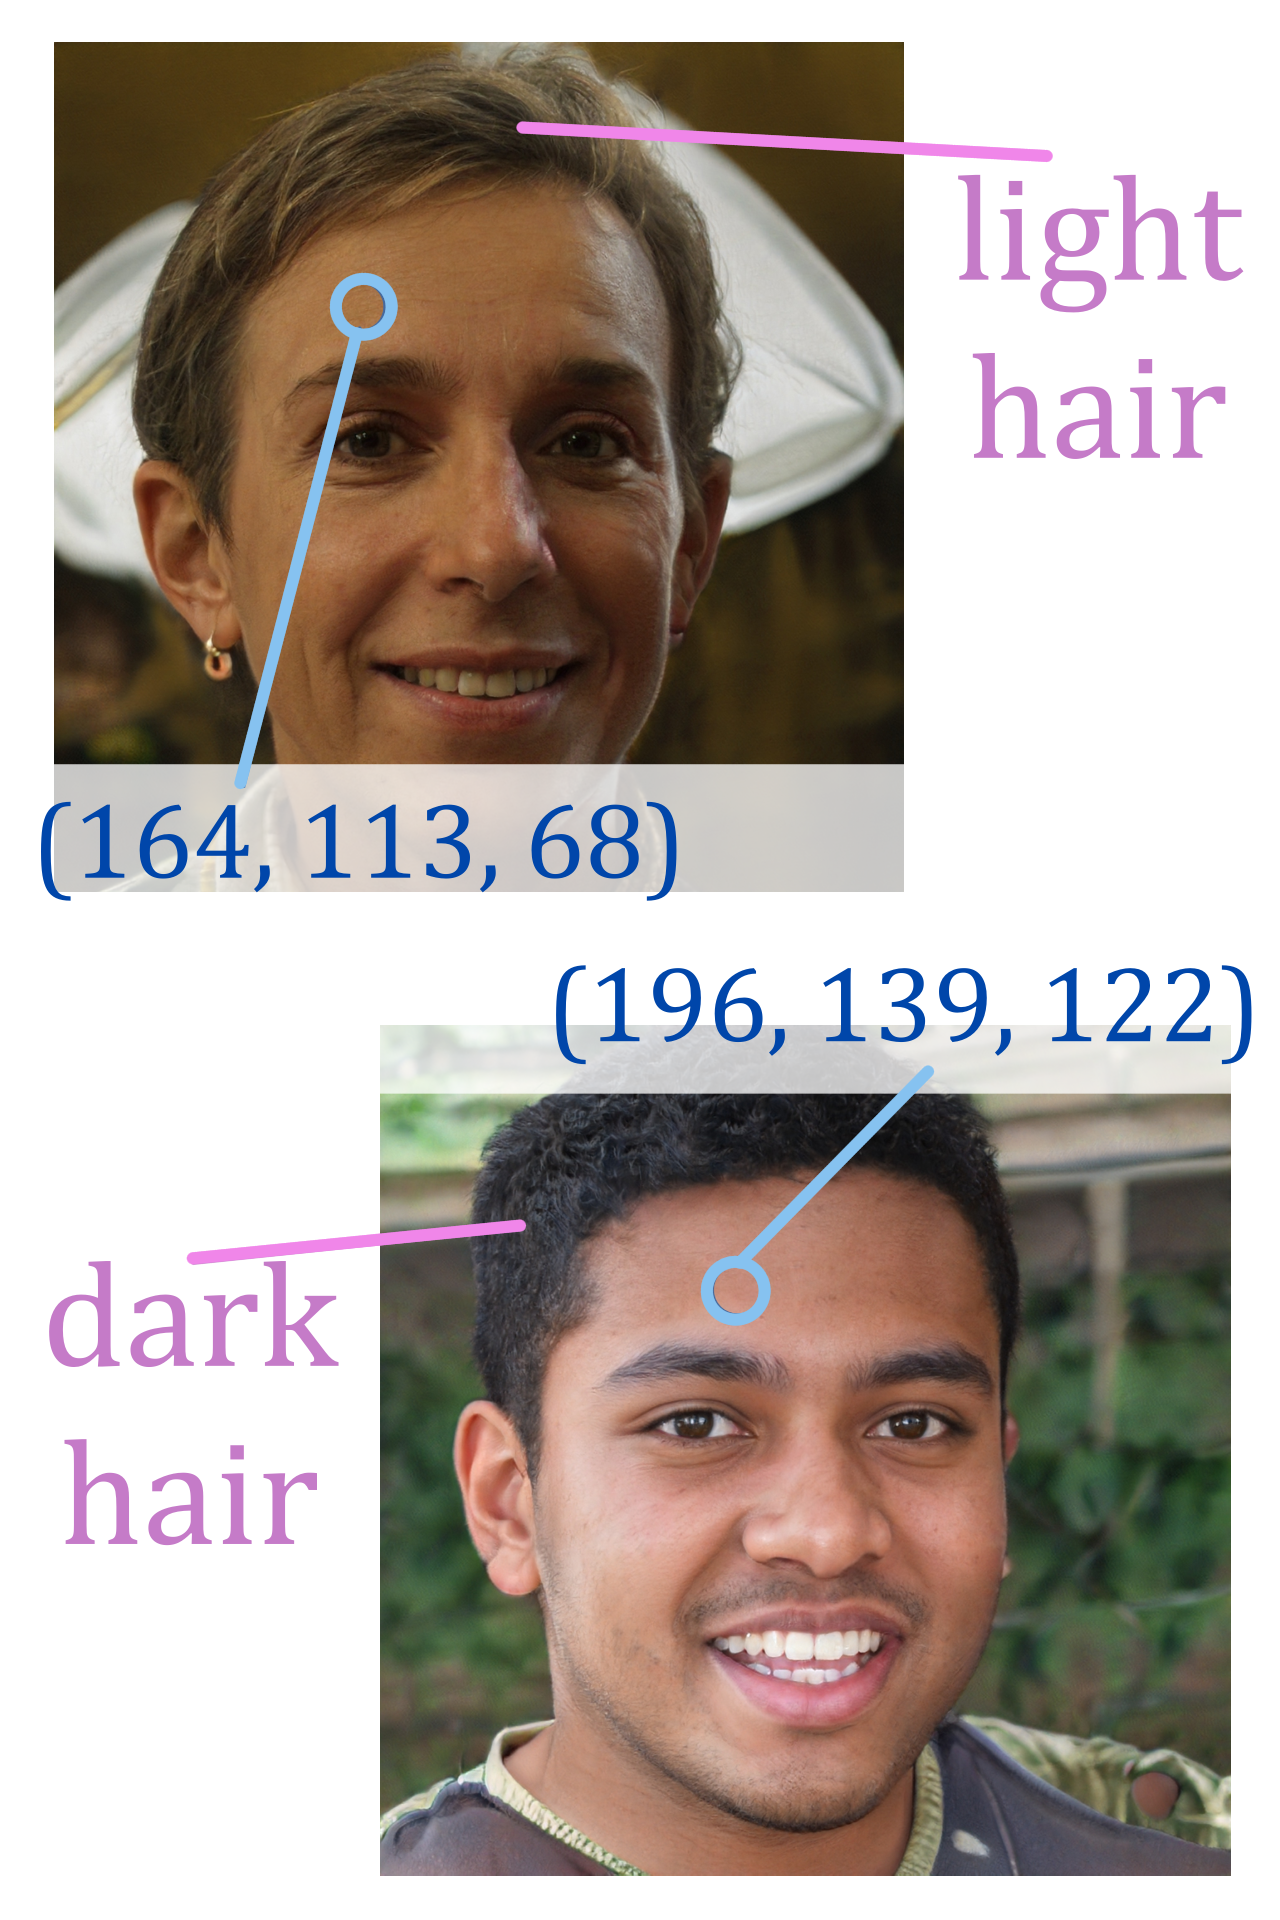
\includegraphics[width=\linewidth]{latentvariables.png}
\caption{\label{fig:latentfaces}Two randomly generated images from \url{https://thispersondoesnotexist.com}. In blue, available features such as the color values of some pixels. In pink, latent variable values (such as \textit{hair tone}) that are not directly represented in the data but influence those color values.}
\end{marginfigure}

Furthermore, the techniques used for collecting data can only produce the observable variables in a dataset, but there may be interesting, hidden variables which influence the data in a clearer way. This is a concept known in statistics as \textit{latent variables} \sidecite{borsboom2008latent}. For example, the value  ``blond'' for the latent variable ``hair color'' might determine the color value of many pixels in an image of a person's face, but those are also influenced by overall lighting and contrast, so the hair color of a person cannot be deduced by just extracting a couple of pixels (see Figure~\ref{fig:latentfaces} for an example). It would be desirable to obtain the meaningful features, but a learning mechanism that takes all observable features into account is needed for these to be extracted.

Providing a learning algorithm with unprocessed features usually leads to sub-par performance due to several potential issues: different scales, presence of noisy variables, redundant information, useful information that is obscured and not directly represented, as well as irrelevant information. All of this may confuse a learning method which initially might consider all variables equally relevant.

Other possible obstacles that one may come across when inspecting the features of a dataset are difficult classes, also known as data complexity \sidecite{cano2013analysis}. This scenario arises when the variables do not provide sufficient information to allow class separation, the relations between variables and the target are highly nonlinear, or other circumstances prevent a learning method from inferring an adequate mapping from the input features to the target variable.

As a consequence, much time can be spent manually engineering features according to what the practitioner believes the learning method will adapt best. However, this is a process that requires experience and usually involves many attempts at improving results. Instead of this, a new task can be performed by machine learning techniques before the actual knowledge extraction, called \textit{feature learning} or more broadly \textit{representation learning} \sidecite{bengio2013representation}. 

Feature learning alleviates a notable amount of manual labor and dataset manipulation although, of course, implies that the user know about feature learning methods and their operation. There exists a very diverse array of methods, ranging from simple principal component analysis (PCA) to more complex manifold learning methods.

However, not every feature learning method can solve every task. Most of them have a specific criterion that they optimize, such as maximum variance in the case of PCA, point reconstruction from its neighbors as in locally linear embedding \sidecite{LLE}, or shortest-path distances between points as in Isomap \sidecite{Isomap}. The objective function of each method determines which behavior will be found in the extracted representation, with little to no room to customize it. There may be situations where it is necessary for the learned variables to adjust to certain properties and, ideally, the feature extraction method should allow to enforce those properties.

\section{Tools}

The main set of tools that are used to tackle problems along this work is \textit{deep learning}, a subset of machine learning focused on algorithms which extract successive transformations of the data until a solution to the task is reached.

Deep learning originates from the concept of artificial neuron, which takes some inspiration on the biological nervous system \sidecite{mcculloch1943logical}. The perceptron, a probabilistic model of the brain, was developed drawing from this abstract neuron \sidecite{rosenblatt1958perceptron} and current artificial neural networks are simply generalizations of the multi-layer perceptron (MLP). For a long time, neural networks were very inefficient to train compared to other machine learning methods, and they were not used for many applications as a result.

The resurgence of neural network models for machine learning has happened more recently due to the fact that their optimization had much higher computational cost than other, classical machine learning models. Thus, more efficient optimization strategies in combination with much more powerful hardware (leveraging the computing capacities of modern GPUs) have allowed to train complex deep models which were unfeasible before.

Nowadays, deep learning is used to extract the contents of images, natural language and speech (as well as produce them) in a wide range of applications, from small fitness devices to autonomous vehicles. It is also very present in research fields ranging from medicine to computer security. It powers translation systems \sidecite{deepl}, search engines \sidecite{SHU19991} and virtual assistants \sidecite{mycroft}. 

The main advantage of deep learning against traditional machine learning methods is being able to automatically transform raw data into useful representations that depict more complex, high-level concepts. This stage is usually performed manually when approaching machine learning problems with other models.

Since deep learning models perform their own representation learning while training to solve other tasks, one possible use for these models is the extraction of said representations. One can either extract these \textit{deep features} from neural networks which are trained for a different purpose or build a deep learning model dedicated to just learning a new, more useful representation. The latter approach will be our focus during most of this thesis, using a specific category of models known as \textit{autoencoders}.

\section{Motivation}

The questions that we are trying to tackle throughout this thesis can be summarized as follows:

\begin{itemize}
    \item How can representation learning be approached with deep neural models?
    \item What benefits can be obtained by transforming data into an appropriate representation?
    \item Can specific behavior be induced within the transformations, such as separating different classes?
\end{itemize}


% - the potential of deep neural models over other methods for feature learning

As the trends in usage of deep learning models to solve machine learning problems continue to increase, we focus our interest in their potential to not only tackle supervised problems such as classification, regression or detection, but also wider problems where solutions are not so easily validated, such as feature learning. Since deep learning allows the integration of the feature extraction stage directly within the predictor itself, these types of models should be valuable feature learners for other tasks as well.

% - interest in how to adapt feature generation for different purposes, e.g. multiple outputs

Deep neural models dedicated to generating new feature sets could be adapted, as a result, to different purposes. For instance, one could search for feature spaces where ``ordinary'' data points are very cohesive, and thus anomalous inputs would be easy to identify. Similarly, a transformation of features could allow for better separation of different classes, better distinction between noise and signal, or more meaningful traits that relate to all the original variables.

% - interest in multi-view problems

Another potential use of feature learning models that catches our interest is the possibility of capturing more than one aspect of each problem instance, which translates to different \textit{views} of the problem, for example, image and text. These views could be processed by different learners or special algorithms, but one could build feature learners that combine the available information into a more machine-ready feature vector.

% - interest in interpretable models

A current conflict of deep learning models with several areas of interest in machine learning, such as medical applications, is the fact that most are essentially black boxes \sidecite{fong2017interpretable}. This means that the behavior of a trained model is obscured by the intrinsic structure and is thus unintuitive for humans to comprehend. As a result, there is much interest in explaining and justifying the behavior of these models. Enabling the use of interpretable classifiers and regressors such as decision trees by means of better dataset representations can be one way of avoiding black boxes in these contexts.

\section{Objectives}

All the research developed along this work has been revolving around the general aim of improving how autoencoders can achieve a better representation of data in order to extract more reliable models from it. 

As a result, the specific objectives that we posed throughout the course of the thesis were the following:

\begin{itemize}
    \item To acquire a deep understanding on how autoencoders work, how they differ from other feature extraction techniques, and the different approaches to learn new features with them.
    \item To facilitate the use of autoencoders by unspecialized users, improving on previous implementations in efficiency and ease of use.
    \item To explore different types of supervised learning problems further from the classical binary (positive/negative) prediction schemes or regression tasks.
    \item In the context of supervised problems, to develop new ways of optimizing autoencoders so that generated features are able to separate different classes better.
\end{itemize}

Additionally, there are several tangential issues that were studied due to the interesting relation to the main topic and the opportunity to work on real world problems. These are as follows:

\begin{itemize}
    \item To identify areas of application where autoencoders are able to provide solutions without the need of additional modelling.
    \item To evaluate and compare different encoder-decoder architectures for different purposes .
    \item To analyze whether ensembling several encoder-decoder methods can provide better solutions.
\end{itemize}

\section{Thesis structure}

This work comprises several original introductory chapters presenting the necessary theoretical concepts and the basics on how these are put to practice, as well as reproductions of five articles published in peer-reviewed journals, each of them related one or more of the previously established goals for this thesis.

The rest of this document is organized as follows: %contains all the needed information to develop the posed questions and provide enough context in order to understand the work that has been realized throughout the thesis.

\begin{itemize}
    \item Chapter~\ref{ch:theory} describes the basic theory that lies under the subsequent works and the specific models that are developed and used.
    \item Chapter~\ref{ch:practical} explains the practicalities of implementing and training deep learning models, especially autoencoders.
    \item Chapter~\ref{ch:summary} outlines the main results obtained during the research period, providing context and connections among the articles that are reproduced next.
    \item Article~\ref{ch:paper1}, the first of the journal articles, is a guide on the inner workings of autoencoders, their variants, how to design and how to implement them.
    \item Article~\ref{ch:paper2} describes into detail the software developed with the objective to facilitate the use of autoencoders.
    \item Article~\ref{ch:paper3} is a review of the current state of the art in supervised learning further from the standard problems.
    \item Article~\ref{ch:paper5} covers the most popular applications of autoencoders apart from classification, with concrete examples and guidelines.
    \item Article~\ref{ch:paper6} improves the applicability of autoencoders in classification problems by developing new loss functions which help reduce data complexity.
    \item Lastly, Chapter~\ref{ch:conclusions} draws some conclusions and closing statements on the developed work.
\end{itemize}